\section{General}\label{sec:general4}
Overall, this project successfully demonstrates a working proof of concept for a foosball robot.
Its main advantage over similar projects lies in the simplicity of the design, which eliminates the need for motor movement.
This simplicity allows for easy expansion to heavier, faster, and stronger motors and enables the construction of the three remaining players.
The core concept and design were well-thought-out, requiring minimal changes during the construction phase.
The goalkeeper can stop slow moving balls with high accuracy.
However at high speeds the software is not sophisticated enough to move the player to the correct position in such a short time.
This is largely because the stepper motor needs multiple iterations of movement and measurement to reach the desired position.
This can be fixed by using the custom PCB provided by the company, which uses the RS485 communication standard.

%\section{Embedded Programming}\label{subsec:results_embedded}
%The code on the Arduino is not as sophisticated as desired.
%While it performs the tasks well enough at low speeds, at higher speeds the motor becomes inconsistent and inaccurate.
%This issue can be resolved with the custom PCB provided by the company, which uses the RS485 communication standard.
%Therefore, this improvement is listed as a future enhancement in Section~\ref{sec:improvements}.

\subsection{Precision}\label{subsec:precision}
The precision has not yet reached $\qty[per-mode=symbol]{1}{\mm}$.
Measuring it precisely is challenging because the closer the player is, the more precise the IR sensor needs to be.
Additionally, the IR sensor occasionally fails to measure the distance correctly, leading to improper movement of the player.

\subsection{Tests}\label{subsec:tests}
To evaluate the precision of the system, I have set up a test environment involving the robot and random ball throws to simulate game conditions where balls are also thrown unpredictably.\\
Initially, I tested slow-moving balls.
Out of $20$ balls, the goalkeeper successfully stopped $14$.
Next, I tested fast-moving balls, with the goalkeeper stopping $10$ out of $20$.
The missed balls were often due to the stepper motor moving too quickly and overshooting its target.
This issue can likely be mitigated by further tuning variables such as the motor's acceleration and deceleration.\\
The first tests using the RS485 communication standard were also promising.
The motor consistently moved to the correct position, albeit at a much slower speed compared to the current implementation.
This slowdown can be addressed by adjusting the PCB settings, which I plan to optimize in future tests.\\
Shooting the ball, while standing still, works very well, which was quite surprising after having made a mistake during the calculations.
During movement, the ball is not always shot at the correct moment in time, which is due to very precise timing required.
This issue is also attributed to camera latency and USB driver delays.
Additionally, the inexpensive physical DC motor driver used is outdated, unable to ramp up speed quickly enough, and prone to overheating.


\section{Image processing and optics}\label{sec:results_image}
The undistortion function works very well, largely due to a high level of iterations of the calibration process.
Ball detection is also highly accurate, successfully detecting only the ball while avoiding the tube or the player.
However, under certain lighting conditions, human hands are occasionally detected as the ball.
This issue could be resolved by using a differently colored ball.\\
Still, the ball prediction is accurate, with a small margin of error.
However, timing inconsistencies remain, where the player sometimes shoots too early or too late.

\section{In Action}\label{sec:in-action}
Figure~\ref{fig:before_catch} and figure~\ref{fig:catch} show a small portion of the frames captured during the ball-catching process.
The left image shows what the program sees through the camera from below and the right one shows the actual scene from above.
As the camera looks from below, the image is mirrored.
\begin{figure}[H]
    \centering
    \begin{subfigure}{.5\textwidth}
        \centering
        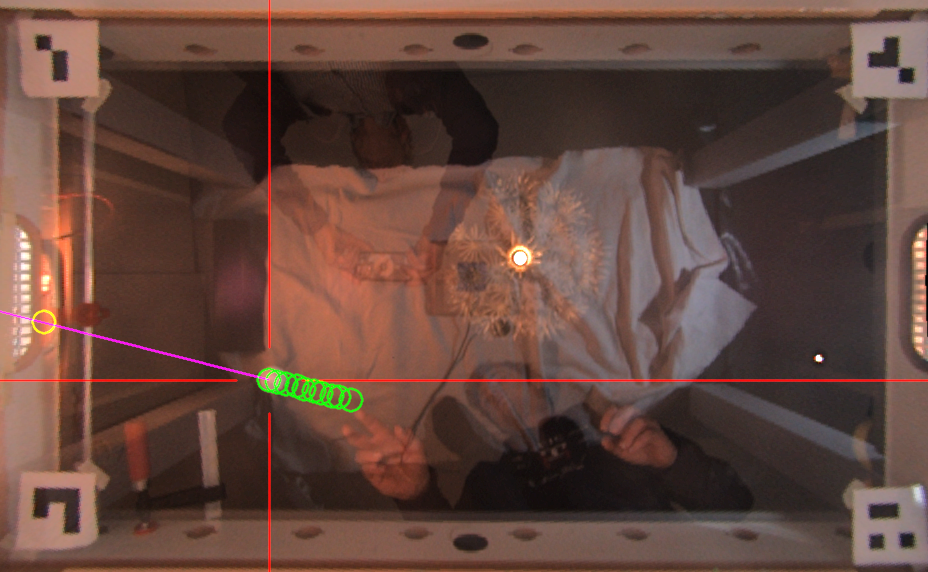
\includegraphics[width=0.9\textwidth]{../photos/player_before_catch_bottom}
        \caption{Image from below with ball detection}
        \label{fig:player_before_catch_bottom}
    \end{subfigure}%
    \begin{subfigure}{.5\textwidth}
        \centering
        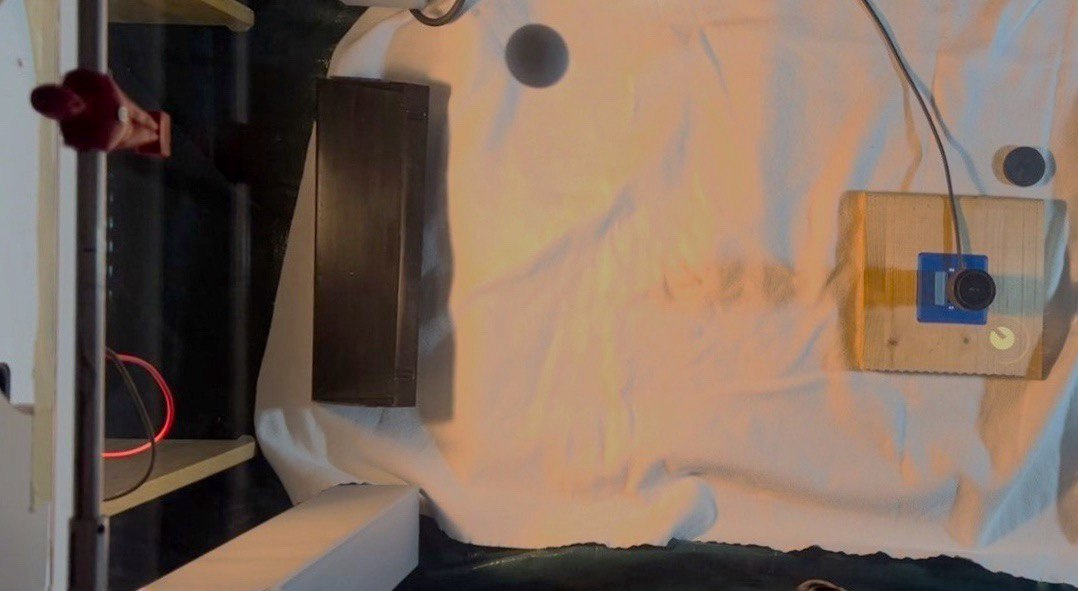
\includegraphics[width=0.9\textwidth]{../photos/before_catch_top}
        \caption{Image from above}
        \label{fig:before_catch_top}
    \end{subfigure}
    \caption{Before catching the ball}
    \label{fig:before_catch}
\end{figure}


\begin{figure}[H]
    \centering
    \begin{subfigure}{.5\textwidth}
        \centering
        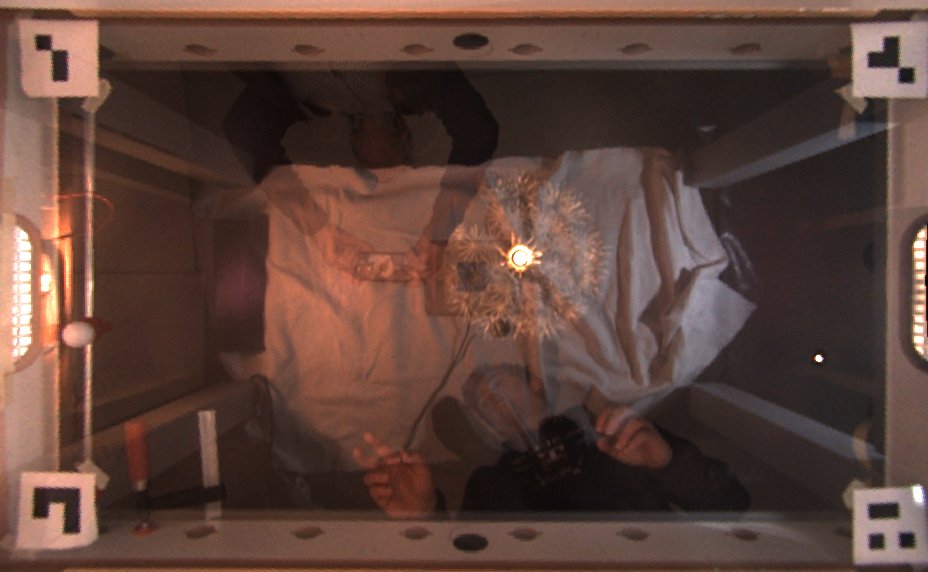
\includegraphics[width=.9\textwidth]{../photos/player_catch_bottom}
        \caption{Image from below (what the program sees)}
        \label{fig:player_catch_bottom}
    \end{subfigure}%
    \begin{subfigure}{.5\textwidth}
        \centering
        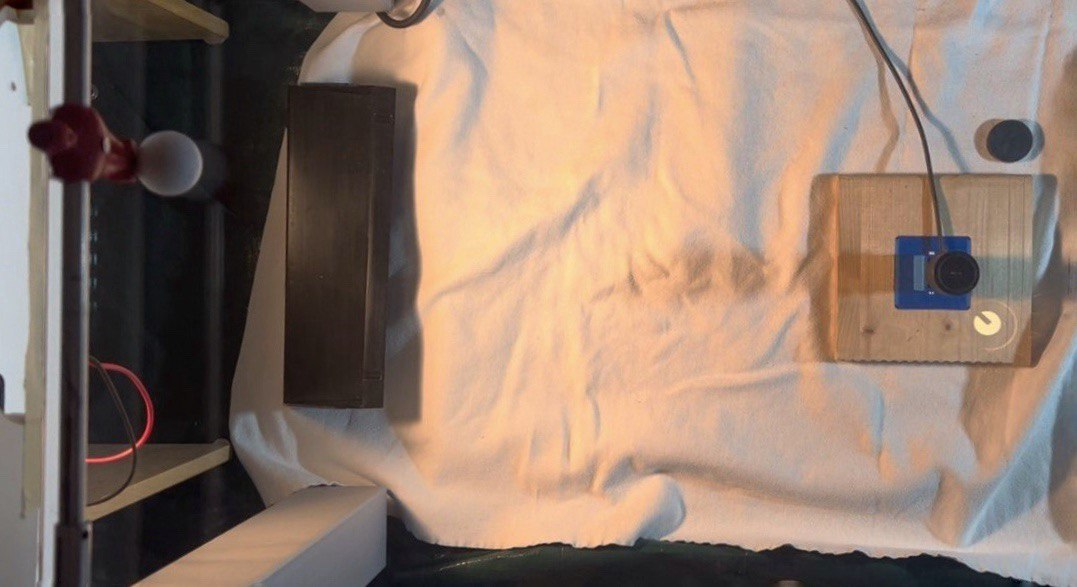
\includegraphics[width=.9\textwidth]{../photos/catch_top}
        \caption{Image from above}
        \label{fig:before_top}
    \end{subfigure}
    \caption{While catching the ball}
    \label{fig:catch}
\end{figure}